\chapter{Introduction to Organisation}\hrule
\label{Chapter:1}
% =====================================================================================================
\section {Organisation Profile and History}

I had my Six Months Training at Auribises Technologies, Ludhiana. Auribises Technologies was founded in Nov, 2011 by Mr. Ishant and some of its colleagues. The company has great fame in training students in Andriod, Java EE, AI, Java SE, Web related technologies across India. It is an ISO 9001-2015 certified company.
\\
\\
The company main motive is to impart the deep programing and computing skills in the students across india in an affordable way. The company also provides online training on various skills like Data Science. It also have experience in training employees of various big corporate IT firms across india.\\
\\
The Institute is at 4 Km driving distance from Ludhiana Junction, located in Krishna Nagar, Ludhiana, Punjab.It is an ISO 9001:2008 certified company. The company has a well equipped lab facility available for its students.
\\
\\
Auribises was founded in 2011 in Ludhiana (India) by Ishant Kumar and has been very successful in the field of software development and IT Training ever since.The core competency of Auribises is the development of software solutions for common problems of users, developers and enterprises. As an IT service provider Auribises develops individual desktop, server, web-based, mobile-based software solutions as requested by the cutomer.
\\
\\
Auribises is a leading technical service provider. Their goal is to be the leading independent provider of technical services for development, consultation and training. Since 2011, They have been developing solutions to ensure the quality and economic efficiency. They firmly believe that social and technological progress is inextricably linked together and implementing the combination Auribises aims to deliver "end user happiness".
\\
\\
Two words that perfectly encapsulate their commitment to service: whatever they do, they do it precisely and they do it right. They use new ideas, technology and expertise for development of products, services, systems and people and make them more competitive. Their Training Services are based on latest technologies which inspire their customers. Team Auribises create optimal software solutions and guarantee high-quality customer support.
\\
\\
The institute has more than 1K students who are trained in various latest software technologies in a year. The company has excellent history in software training and the company is also keenly looking forward to continue its legacy.

\chapter{Introduction to Project}\hrule
\label{Chapter:2}
% =====================================================================================================
\section{Overview}

MilkDiary aims to solve one of the biggest problems of the MilkMan across the country. The main tension of MilkMen are keeping the calculation update of the customers. This app will help MilkMen to keep track of their product delivery and total income per consumer. \\
\\
While developing the project, i followed the industry standards of MVP i.e Model View Presenter model. It follows the software engineering principles of low coupling and high cohesion. This model is followed to develop better softwares and to maintain a sustianable software product for a longer period of time.\\
\\
\textbf{What is MVP model?}\\
The MVP pattern allows separate the presentation layer from the logic, so that everything about how the interface works is separated from how we represent it on screen. \\
\\
Ideally the MVP pattern would achieve that same logic might have completely different and interchangeable views.\\
\\
First thing to clarify is that MVP is not an architectural pattern, it’s only responsible for the presentation layer . In any case it is always better to use it for your architecture that not using it at all.\\
\\
\textbf{Why use MVP?}\\
In Android we have a problem arising from the fact that Android activities are closely coupled to both interface and data access mechanisms. We can find extreme examples such as CursorAdapter, which mix adapters, which are part of the view, with cursors, something that should be relegated to the depths of data access layer .

For an application to be easily extensible and maintainable we need to define well separated layers. What do we do tomorrow if, instead of retrieving the same data from a database, we need to do it from a web service? We would have to redo our entire view .

MVP makes views independent from our data source. We divide the application into at least three different layers, which let us test them independently. With MVP we are able to take most of logic out from the activities so that we can test it without using instrumentation tests.\\

While developing the project the main focus was that how the app will keep track of its customers and their transactions. Different API and their standard methods has been used to ensure that the app works superbly. Different latest android concepts like floating action bar also have been used in the project in order to have it a beautiful UI.\\
\\
The app will first take rate, quantity of milk, System date as input and will calculate bill based upon Milk and Rate per litre as input by the MilkMan. The main challenge in the project was to implement cloud computing technologies to store database and to perform all operations related to database for the project. To solve the problem, i used \textbf{Google Firebase} , \textbf{Google Firestore}  powered by \textbf{Google Cloud Platform} to track MilkMan and User data requirements.I also used different \textbf{Open Source} libraries like \textbf{TedPermissions}, \textbf{Circular Image View} etc.\\

Whenever MilkMan creates its account, a record is created in Firebase backend.Then the application's Main Activity is opened. In Main Activity, MilkMan will add its users,whenever MilkMan gives milk to the user, it will input the Quantity of Milk given and the rate of milk per litre. MilkMan can View the transaction History and Grand total. MilkMan can also delete the transaction history if he wants, anytime.\\
\\
Future of the app is very bright.It will be a game changer in increasing the income of Milk Farmers and will surely Digitize the milk transportation chain in our country. I hope the app will reach new heights in future and will solve and increase the revenue of Milk Farmers.
\section{Existing System}

No such type of Independent App exists but on \textbf{Dec 10, 2017}  in an event in \textbf{Banglore, India} a \textbf{Startup} company named \textbf{MilkMan} has been evaluated as \textbf{20 Million USD} . The company has been granted a fund of \textbf{1 Million USD} to complete its inital target for 2018.  \textbf{My MilkDiary app is a part of idea of the fully featued App, but the company's app is yet to be developed} . \\
\section{User Requirement Analysis}
\subsection{What is the Problem?}
In this digital world, our Milkmen are still using that age old diary techniques to save our transaction history manually. I thought that this process can be automated and will rescue the Milkman from hectic calculation tasks. A milkman can also get more number of customer base to interact with and can increase its income by delivering milk to them.
\subsection{Why is it important to solve the problem?}
\begin{itemize}
	\item There is a chance to do mistake while making calculations as most of the MilkMan are not fully qualified.
	\item As, the diary is always with the milkman, there is a chance of anomaly. The milkman may be greedy and could change the quantity of milk, rate or diary entries which may lead to a bad Milkman-customer relationship.
	\item So, An app is necessary to help Milkman and Customers both.  
\end{itemize}
  
\subsection{Requirements Gathering}
Requirements gathering is also popularly known as requirements elicitation. The primary objective of the requirement gathering task is to collect the requirements from the stakeholders.\\
A stakeholder is a source of requirements and is usually a person, or a group of persons who either directly or indirectly are concerned with the software.\\
\\
Procedures adopted while requirements gathering during the project were:
\begin{itemize}
	\item \textbf{Interview:} Around 10 MilkMan were interviewed for the gathering their requirements.
	\item \textbf{Scenerio Amalysis:} The different use cases and functionality of the app were discussed. It includes the discussion on Main panel and followed by transaction history for a MilkMan.
	\item \textbf{Task Analysis:} The technologies to be used in Frontend anf Backend were discussed.
	\item \textbf{Form Analysis:} We formed a yes no tick mark questionaire for the MilkMan and some for the Customer to analyze their requirements.
	\item \textbf{Studying Documentation}: The documentation of various cloud technologies were studied and discussed with the Project Mentor. Finally, we agreed on using \textbf{Google Firebase} and \textbf{Google Cloud Platform} as our cloud technology.
\end{itemize}
\subsection{Functional Requirements}
\begin{itemize}
	\item MilkMan and Customers need an Android phone with good internet connection.
	\item Android phone needs to have atleast 1 GB Ram and atleast 2GB of external usable memory.
	\item Android phone should have android os version "Kit-Kat" or above.
\end{itemize}
\section{Feasibility Study}
A feasibility study is used to determine the viability of an idea, such as ensuring a project is legally and technically feasible as well as economically justifiable. It tells us whether a project is worth the investment—in some cases, a project may not be doable. There can be many reasons for this, including requiring too many resources, which not only prevents those resources from performing other tasks but also may cost more than an organization would earn back by taking on a project that isn’t profitable.\\
\\
The application is fully feasible. It just needs a working internet connection,a gps and android 4.0 and above. It is fully feasible if it is also deployed on a large scale.\\
The application can also be upgraded further and can be deployed on large scale depending upon the need of business plan.\\
\begin{enumerate}
	\item \textbf{Technical Feasibility :} The app is fully feasible on technical terms. I have android studio and required 8 GB Ram for development purpose.\\
	I will use Firebase cloud to deploy backend as it is free for inital and small projects.\\
	The version control system is completely free and the website Github.com is also free for Open Source Projects.
   \item \textbf{Economic Feasibility :} The app is fully economically feasible as it has free and open source tools being used while developing the system.\\
   The Firebase Cloud technology is free till 10K hits in a day. So, intially around 6-7 months after releasing the project, it is expected to have a user base of around 10K people. Later on, If the user base increases, the revenue of product will also increase and further resources can be purchased.
   \item \textbf{Legal Feasibility :} The app doesn't violates any legal rights and will credit the author of open Source Library used while developing the project.\\
   The project will be available in open source under \textbf{GPLv3} license.\\
   \\
   \textbf{What is GPLv3 License?}
   \begin{itemize}
   	\item The source code must be made public whenever a distribution of the software is made.
   	\item Modifications of the software must be released under the same license.
   	\item Changes made to the source code must be documented.
   	\item If patented material was used in the creation of the software, it grants the right for users to use it. If the user sues anyone over the use of the patented material, they lose the right to use the software.\\
   \end{itemize}
 
   \item \textbf{Operational Feasibility : } As the app satisfies the functional and non functional requirements, the app will be fully operational once it releases.
   
   \item \textbf{Scheduling Feasibility : } The project release targets for different versions are practical and have plenty of time develop and debug the app before release.
\end{enumerate}

\section{Objectives of the Project }
\begin{itemize}
	\item The project is developed to give a solution and to the digitalize the Milk Delivery chain.
	\item The main motive behind developing the project is to rescue the MilkMan from hectic calculations. The app will help MilkMan to increase their revenue.
	\item The app will help MilkMan customers to track on their milk based products expenditures and in future, will deliver milk products on demand.
	\item From the developer side, the app will generate revenue based on Google Adwords from free tier Users and will charge a very small monthly amount (hardly 10-20 INR) form premium MilkMan account holders.
\end{itemize}


\chapter{Product Design}\hrule
\label{Chapter:3}
% =====================================================================================================

\section{Product Perspective}
The application will have a user friendly and menu based interface.Following screens will be provided:
\begin{itemize}
	\item A Login Screen.
	\item A Signup Screen.
	\item A Reset password screen.
	\item Two floating action button.
	\item One FAB to create user and other to delete their transaction .
	\item One menu button to Logout the user.
	\item One alert dialogue will be generated before deletion of transaction by the MilkMan.
	\item Alert dialogue will have 2 buttons. One having "Yes" option and other having "No" option.
	\item After clicking on "Yes" the transaction history will be deleted from transaction history and from firebase realtime database.\\
\\	
	
\end{itemize}
\section{Product Functions}
\begin{itemize}
	\item MilkMan can input Quantity and rate manually.
	\item MilkMan can add Customers.
	\item MilkMan needs to click Logout options menu to Logout from the app.
	\item App will calculate amount of money to be paid per day automatically
	\item App will calculate Grand total of the transaction automatically
	\item MilkMan needs to click delete FAB in order to delte transactions history.\\
	
\end{itemize}
\subsection{Functional Flow}
\textbf{In version "1.0"  :} (to be released by Dec 30,2017)
\begin{itemize}
	\item MilkMan need to create its account.
	\item MilkMan can login.
	\item MilkMan can add Customers.
	\item MilkMan can see the transaction history.
	\item MilkMan can delete the transaction history.
\end{itemize}
\textbf{In version "1.1" :} (to be released by Jan 15,2018)
\begin{itemize}
	\item MilkMan can remove users.
	\item MilkMan can generate bills in form of pdf and can send bill to customers.\\
\end{itemize}
\textbf{In version "1.5" :} (to be released by Feb 28,2018)
\begin{itemize}
	\item \textbf{Paytm Payment Gateway} will be integrated to recieve payments.
	\item A new user module to be added, where customers can register themselves, Login and can see their transaction history from their respective MilkMan.
\end{itemize}
\textbf{In version "2.0" :} (to be released by Apr 15,2018)
\begin{itemize}
	\item Customers can see different milkmen delivering milk to their nearby locations.
	\item Customers can send a request to MilkMan to deliver milk to them.
	\item Customers can rate and write reviews about the Milkmen to whom they have been a customer in the past.   
\end{itemize}
\section{User characteristics}
MilkMan will get a floating action button to add customer and On clicking the name of the user, transaction History will be shown.\\
MilkMan needs to submit Quantity and Rate manually while date will be automatically handled by the app.\\
MilkMan needs to click delete FAB to delete transaction history .
\section{Constraints} 
\begin{itemize}
	\item User needs Android 4.4 i.e "KitKat" and above.
	\item User needs active internet connection.
	\item User have to set Quantity and rate at the time of delivering the milk.
	\item Total of the day and Grand Total will be Calculated automatically.
\end{itemize}
\section{Flow Chart}
When user opens the app,does he Login or SignUp?\\
If yes, he is directed to Main Screen. If no, user is on Same Screen.\\
User creates the user profile.\\
User inputs the Quantity and rate, then he is directed  to the show transactions activity.\\
He click the FAB to delete transactions, transaction is deleted .
\begin{figure}[h]
	\centering
	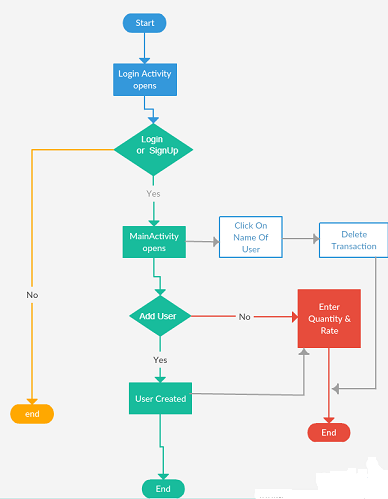
\includegraphics[width=0.75\linewidth]{flowchart}
	\caption{Control flow diagram}
	\label{fig:flowchart}
\end{figure}
\section{Database Design}
The database is a NoSQL Database. The data is stored in Tree data structure.\\
\subsection{NoSQL Database}
\textbf{What is NoSql Database?}\\
\\
NoSQL is an approach to database design that can accomodate a wide variety of data models, including key-value, document, columnar and graph formats. NoSQL, which stand for "not only SQL," is an alternative to traditional relational databases in which data is placed in tables and data schema is carefully designed before the database is built. NoSQL databases are especially useful for working with large sets of distributed data.\\
\subsection{NoSQL vs. RDBMS}
The NoSQL term can be applied to some databases that predated the relational database management system, but it more commonly refers to the databases built in the early 2000s for the purpose of large-scale database clustering in cloud and web applications. In these applications, requirements for performance and scalability outweighed the need for the immediate, rigid data consistency that the RDBMS provided to transactional enterprise applications.

Notably, the NoSQL systems were not required to follow an established relational schema. Large-scale web organizations such as Google and Amazon used NoSQL databases to focus on narrow operational goals and employ relational databases as adjuncts where high-grade data consistency is necessary.

Early NoSQL databases for web and cloud applications tended to focus on very specific characteristics of data management. The ability to process very large volumes of data and quickly distribute that data  across computing clusters were desirable traits in web and cloud design. Developers who implemented cloud and web systems also looked to create flexible data schema -- or no schema at all -- to better enable fast changes to applications that were continually updated.\\
\textbf{Key-value stores}\\
Key-value stores, or key-value databases, implement a simple data model that pairs a unique key with an associated value. Because this model is simple, it can lead to the development of key-value databases, which are extremely performant and highly scalable for session management and caching in web applications. Implementations differ in the way they are oriented to work with RAM, solid-state drives or disk drives. Examples include Aerospike, Berkeley DB, MemchacheDB, Redis and Riak.\\
\textbf{Document Databases}\\
Document databases, also called document stores, store semi-structured data and descriptions of that data in document format. They allow developers to create and update programs without needing to reference master schema. Use of document databases has increased along with use of JavaScript and the JavaScript Object Notation (JSON), a data interchange format that has gained wide currency among web application developers, although XML and other data formats can be used as well.  Document databases are used for content management and mobile application data handling. Couchbase Server, CouchDB, DocumentDB, MarkLogic and MongoDB are examples of document databases.\\
\textbf{Wide-column stores}\\
Wide-column stores organize data tables as columns instead of as rows. Wide-column stores can be found both in SQL and NoSQL databases. Wide-column stores can query large data volumes faster than conventional relational databases. A wide-column data store can be used for recommendation engines, catalogs, fraud detection and other types of data processing.  Google BigTable, Cassandra and HBase are examples of wide-column stores.\\
\textbf{Graph stores}\\
Graph data stores organize data as nodes, which are like records in a relational database, and edges, which represent connections between nodes. Because the graph system stores the relationship between nodes, it can support richer representations of data relationships. Also, unlike relational models reliant on strict schemas, the graph data model can evolve over time and use. Graph databases are applied in systems that must map relationships, such as reservation systems or customer relationship management. Examples of graph databases include AllegroGraph, IBM Graph, Neo4j and Titan.\\
\textbf{Evolution of NoSQL}\\
Berkeley DB was an influential system in the early evolution of NoSQL database usage. Developed at the University of California, Berkeley, beginning in the 1990s, Berkeley DB was widely described as an embedded database that closely supported specific applications' storage needs. This open source software provided a simple key-value store. Berkeley DB was commercially released by Sleepycat Software in 1999. The company was later acquired by Oracle in 2006. Oracle has continued to support open source Berkeley DB.\\
Other NoSQL databases that have gained prominence include cloud-hosted NoSQL databases such as Amazon DynamoDB, Google BigTable, as well as Apache Cassandra and MongoDB.\\
The basic NoSQL database classifications are only guides. Over time, vendors have mixed and matched elements from different NoSQL database family trees to achieve more generally useful systems. That evolution is seen, for example, in MarkLogic, which has added a graph store and other elements to its original document databases.  Couchbase Server supports both key-value and document approaches.  Cassandra has combined key-value elements with a wide-column store and a graph database. Sometimes NoSQL elements are mixed with SQL elements, creating a variety of databases that are referred to as multimodel databases. 

\section{E-R Diagrams}
\begin{figure}[h]
	\centering
	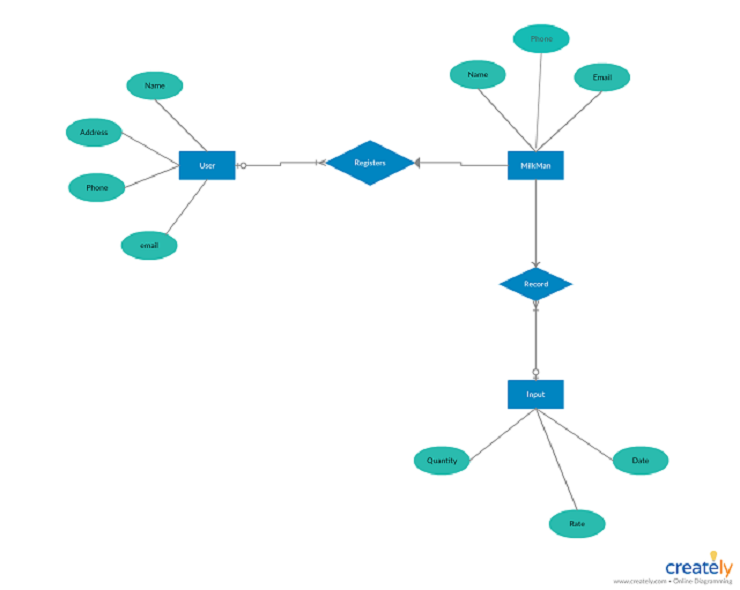
\includegraphics[width=0.75\linewidth]{erdiagram}
	\caption{E-R diagram}
	\label{fig:erdiagram}
\end{figure}

\section{Assumptions and Dependencies}
\begin{itemize}
	\item User is assumed to be using Android 4.4 and above.
	\item User is assumed to have working internet connection.
	\item Grand Total is dependent on the rate and Quantity entered by the user.
	\item Date is dependent on system time. 
	\item Transaction history can be only be deleted once agreed by the MilkMan. \\
	\\
\end{itemize}
\section{Specific Requirements}
\begin{itemize}
	\item Android 4.4 and above.
	\item Working internet connection.
	\item Minimum 1 GB Ram and 2 GB external memory.
\end{itemize}
\chapter{Development and Implementation}\hrule
\label{Chapter:4}
% =====================================================================================================
\section{Introduction to Languages}
\subsection{Front End}
\textbf{XML}\\
XML is used as to design beautiful UI to give user a beautiful experience. Now a days, an app business is more dependent on how interactive, beautiful and simple your UI is.\\
Extensible Markup Language (XML) is used to describe data. The XML standard is a flexible way to create information formats and electronically share structured data via the public Internet, as well as via corporate networks.\\
XML code, a formal recommendation from the World Wide Web Consortium (W3C), is similar to Hypertext Markup Language (HTML). Both XML and HTML contain markup symbols to describe page or file contents. HTML code describes Web page content (mainly text and graphic images) only in terms of how it is to be displayed and interacted with.\\
XML data is known as self-describing or self-defining, meaning that the structure of the data is embedded with the data, thus when the data arrives there is no need to pre-build the structure to store the data; it is dynamically understood within the XML. The XML format can be used by any individual or group of individuals or companies that want to share information in a consistent way. XML is actually a simpler and easier-to-use subset of the Standard Generalized Markup Language (SGML), which is the standard to create a document structure.\\
The basic building block of an XML document is an element, defined by tags. An element has a beginning and an ending tag. All elements in an XML document are contained in an outermost element known as the root element. XML can also support nested elements, or elements within elements. This ability allows XML to support hierarchical structures. Element names describe the content of the element, and the structure describes the relationship between the elements.\\
An XML document is considered to be "well formed" (that is, able to be read and understood by an XML parser) if its format complies with the XML specification, if it is properly marked up, and if elements are properly nested. XML also supports the ability to define attributes for elements and describe characteristics of the elements in the beginning tag of an element.\\
Applications for XML are endless. For example, computer makers might agree upon a standard or common way to describe the information about a computer product (processor speed, memory size, and so forth) and then describe the product information format with XML code. Such a standard way of describing data would enable a user to send an intelligent agent (a program) to each computer maker's Web site, gather data, and then make a valid comparison.\\
XML's benefits sometimes appeared revolutionary in scope shortly after it was introduced. However, as a concept, it fell short of being revolutionary. It also fell short of being the panacea. The over-application of XML in so many areas of technology diminished its real value, and results in a great deal of unnecessary confusion. Perhaps most damaging is the predictable behavior of many vendors that look to recast XML using their own set of proprietary extensions. Although some want to add value to XML, others seek only to lock in users to their products.\\
XML's power resides in its simplicity. It can take large chunks of information and consolidate them into an XML document ‑ meaningful pieces that provide structure and organization to the information.\\
\textbf{Java}\\
In the back end,JAVA is used. Collection and Genrics concepts are mainly used. Java is one of the world's most important and widely used computer languages, and it has held this distinction for many years. Unlike some other computer languages whose influence has weared with passage of time, while Java's has grown.\\

As of 2016, Java is one of the most popular programming languages in use, particularly for client-server web applications, with a reported 11 million developers using and working on it.\\
Applications of java:\\
Java is widely used in every corner of world and of human life. Java is not only used in softwares but is also widely used in designing hardware controlling software components. There are more than 930 million JRE downloads each year and 3 billion mobile phones run java.\\
Following are some other usage of Java :
\begin{itemize}
	\item Developing Desktop Applications.
	\item Web Applications like Linkedin.com, Snapdeal.com etc.
	\item	Mobile Operating System like Android.
	\item	Embedded Systems.
	\item Robotics and games etc.
\end{itemize}
\textbf{Android Platform}\\
The Android platform is an open source mobile development platform. It gives you access to all aspects of the mobile device that it runs on, from low level graphics, to hardware like the camera on a phone. With so many things possible using Android, you might wonder why you need to bother with XML. It is not that working with XML is so interesting, it is working with the things that it enables. XML is commonly used as a data format on the Internet. If you want to access data from the Internet, chances are that the data will be in the form of XML. If you want to send data to a Web service, you might also need to send XML. In short, if your Android application will leverage the Internet, then you will probably need to work with XML. Luckily, you have a lot of options available for working with XML on Android.
\subsection{Back End}
\textbf{Firebase}\\
Web and mobile application often require back-end code to execute tasks like: sending out notifications or processing long running tasks (e.g. scaling images etc). In the traditional approach this back-end code is running on a server.\\
Recently Google’s Firebase introduces a new functionality which is called Cloud Functions. With this new service Firebase offers a scaleable solution for running back-end code in the cloud. Running code in the cloud has various advantages:
\begin{itemize}
	\item You do not need to run and maintain your own server.
	\item You do have an isolated code base for back-end code.
	\item You only get billed for the actual executing time of you code.
	\item The cloud infrastructure is highly scaleable.\\
\end{itemize}
\textbf{Triggers}\\
The functions you write can respond to events generated by Firebase and Google Cloud features. We will call these features triggers. Before starting to develop our first cloud functions let’s explore the most common triggers you can use for Cloud Functions in the following.\\
\\
\textbf{Realtime Database Triggers}\\
With Realtime Database Triggers we’re able to respond to changes in the Firebase Realtime Database. To do so we need to register for events on a specific database path like:

functions.database.ref('/foo/bar')\\
The functions.database.ref function is called and the database path we would like to register for is passed in as a parameter.

It’s also possible to define a part of the path as a wildcard by surrounding this part with curly braces, like you can see in the following:

functions.database.ref('/profiles/{userID}')\\
If you’re just using the ref function, your registering for all events which are write, create, update and delete. If you just want to subscribe to one event you can use the following functions in addition:

onWrite(): is activated when the data is created, destroyed, or changed\\
onCreate(): is activated when new data is created\\
onUpdate(): is activated when data is updated\\
onDelete(): is activated when data is deleted\\
E.g. if we only want a cloud function to be executed if a new user profile unter /profiles/ is created we’re able to register an event handler with the following code:

exports.newUserCreated = functions.database.ref('/messages/{userID}').onCreate(event => { ... });\\
In this case the userID value can be accessed with event.params.userID inside the event handler function.

\section{Supporting Languages}
Follwing API are used:
\begin{itemize}
	\item CircularImageView API.
	\item TedPermissions API for Android.
	\item FirebaseUI.
	\subsection{GIT}
	what is Git? Why Git? What makes Git so popular? We have the answers to all your questions. Just read on!
	
	Git is a Version Control System (VCS), a tool which is an extremely smart choice to use even if it sounds too overwhelming. Simply put, a VCS is a group of files with monitored access. What does that mean? Let's consider a small example to help you understand.
	
	If you are a graphic or web designer and want to keep every version of an image or layout (which you would most certainly want to), a VCS is a very wise thing to use. It allows you to revert files back to a previous state, revert the entire project back to a previous state, compare changes over time, see who last modified something that might be causing a problem, who introduced an issue and when, and more. Using a VCS also generally means that if you screw things up or lose files, you can easily recover. In addition, you get all this for very little overhead.
	
	Many people's version-control method of choice is to copy files into another directory (perhaps a time-stamped directory, if they're clever). This approach is very common because it is so simple, but it is also incredibly error prone. It is easy to forget which directory you're in and accidentally write to the wrong file or copy over files you don't mean to.
	\subsection{Android Studio}
	It’s an Android focused IDE, designed specially for the Android development. It was launched on 16th May 2013, during Google I/O 2013 annual event. Android studio contains all the Android sDK tools to design, test, debug and profile your app. By looking at the development tools and environment, we can its similar to eclispe with the ADT plug-in but as I have mentioned above its android focused IDE, there are many cool features available in Android Studio which can foster and increase your development productivity.
	
	One great thing is that it depends on the IntelliJ Idea IDE which is proved itself a great IDE and has been using by most all the Android engineers.\\
	\textbf{From Where to download?}\\
	You can download Android Studio from the android developer site:\\ http://developer.android.com/sdk/installing/studio.html
	\\
	\textbf{Gradle Build System}\\
	Android Studio uses Gradle as the foundation of the build system, with more Android-specific capabilities provided by the Android plugin for Gradle. This build system runs as an integrated tool from the Android Studio menu, and independently from the command line. You can use the features of the build system to do the following:
	\begin{itemize}
		\item Customize, configure, and extend the build process.
		\item Create multiple APKs for your app, with different features using the same project and modules.
		\item Reuse code and resources across sourcesets.
	\end{itemize}
\end{itemize}
Along with these API, some inbuilt methods of android sdk and Java are also used.
\section{Implementation with ScreenShots}
	First the Login Activity opens.\\
\begin{figure}[h]
	\centering
	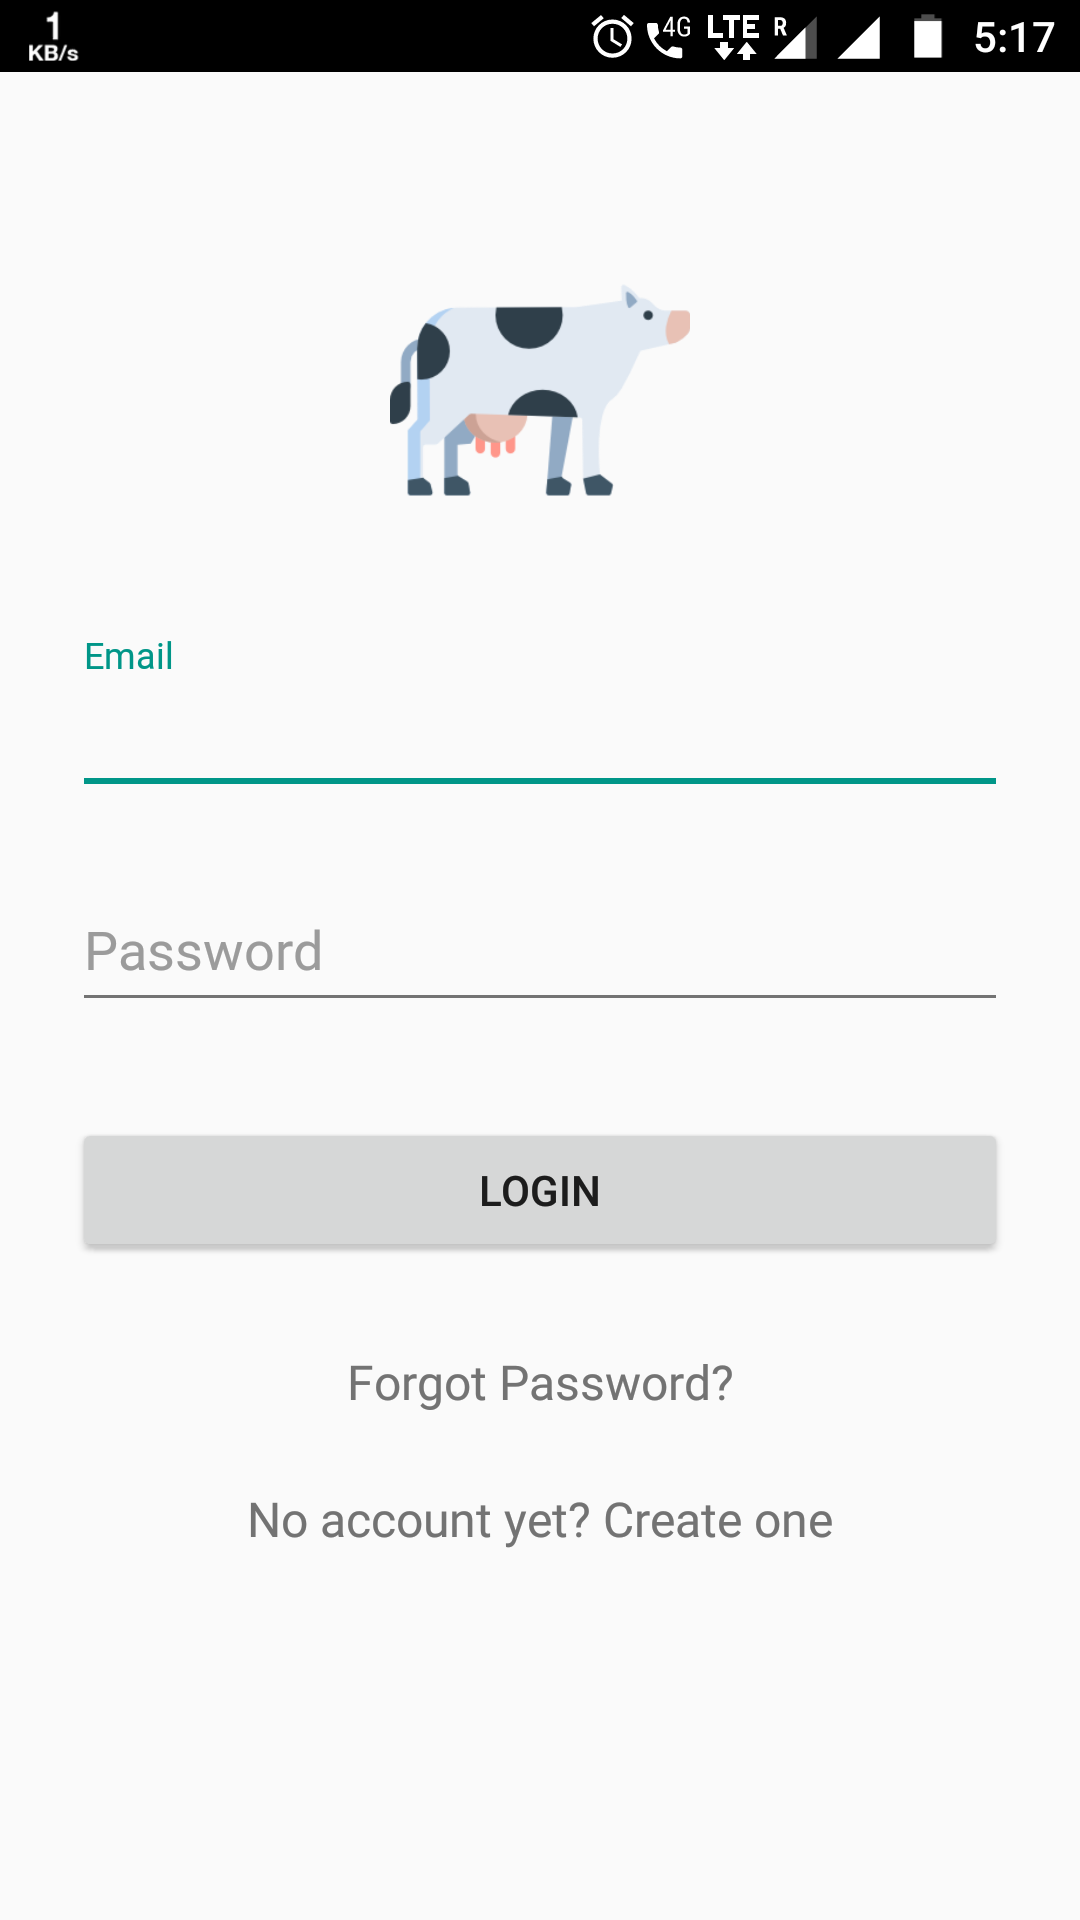
\includegraphics[width=0.7\linewidth]{s01}
	\caption{Login Activity}
\end{figure}
\\
SignUp Activity Looks Like this.

\begin{figure}[h]
\centering
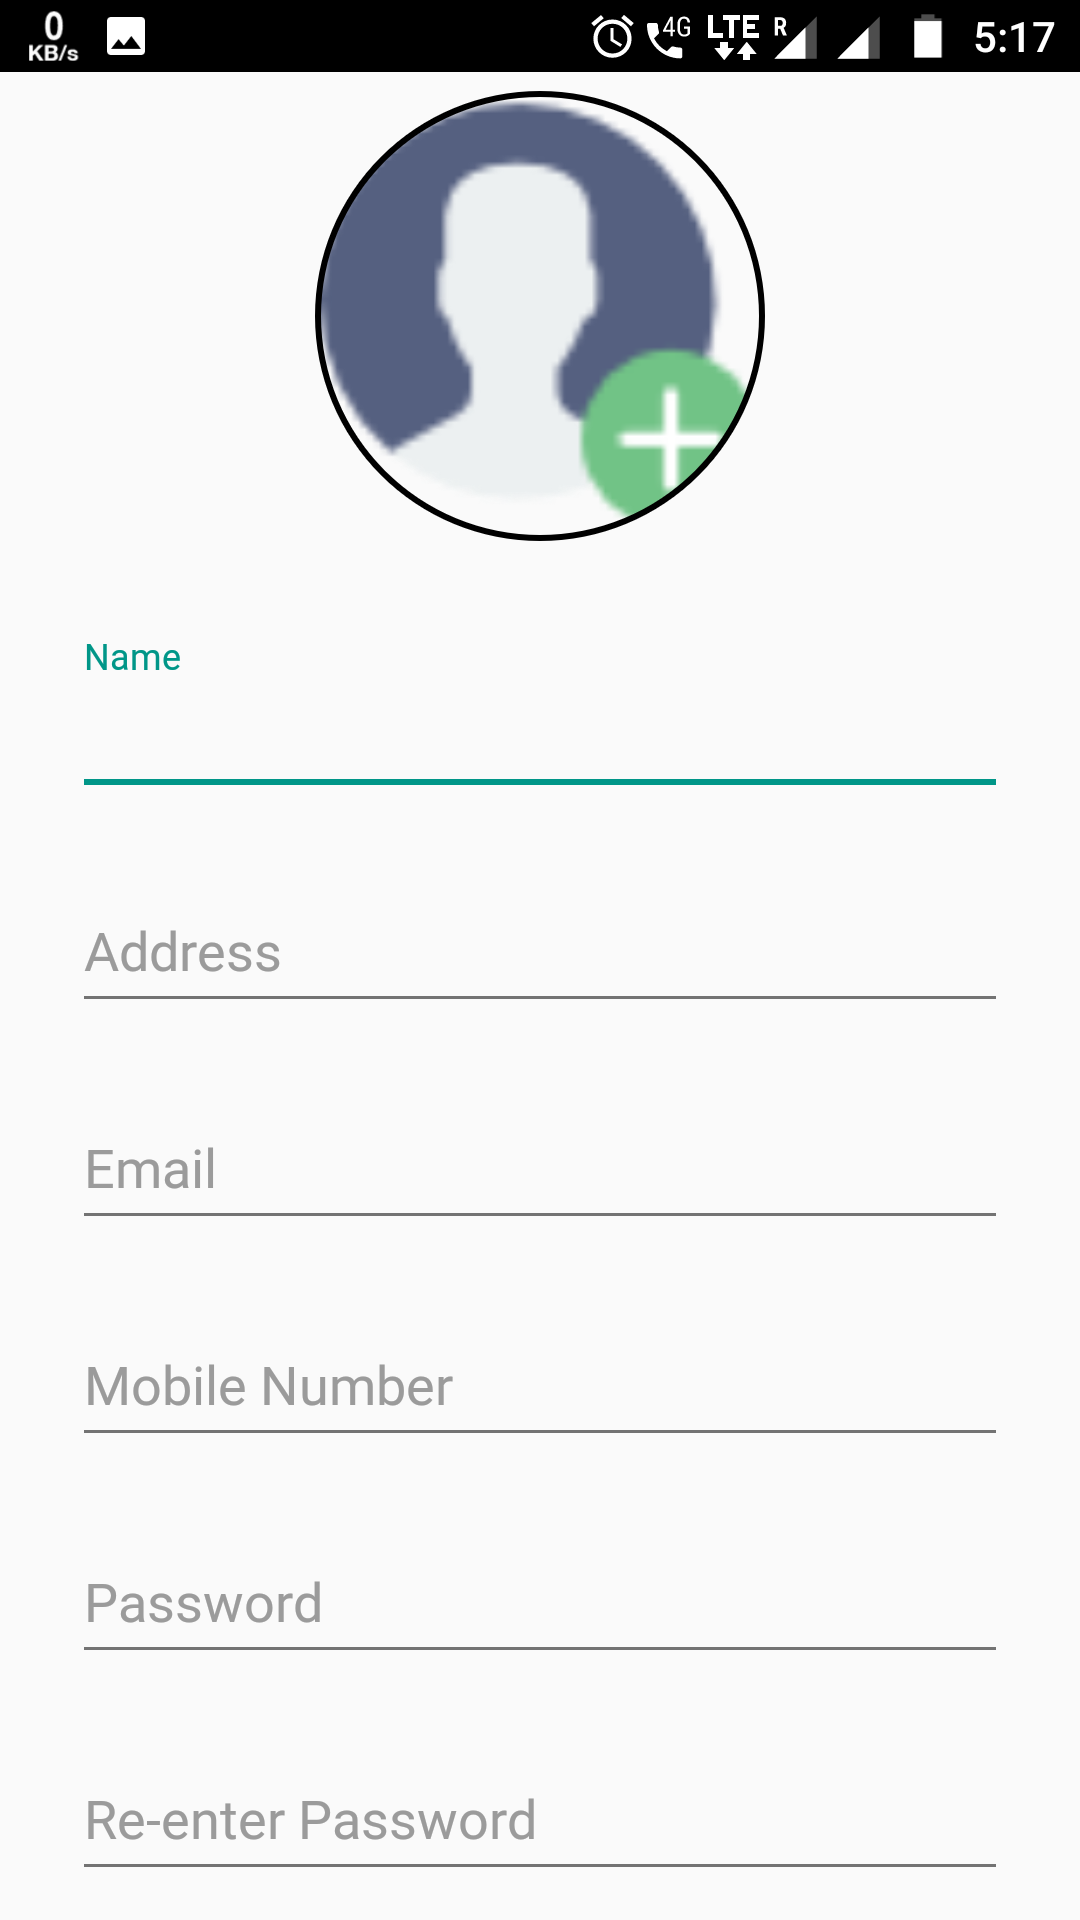
\includegraphics[width=0.7\linewidth]{s02}
\caption{SignUp activity}\\
\\
\end{figure}
\begin{text}
	\\
	\\
	\\
\end{text}	
Forgot Password Activity looks like this
\begin{figure}[h]
	\centering
	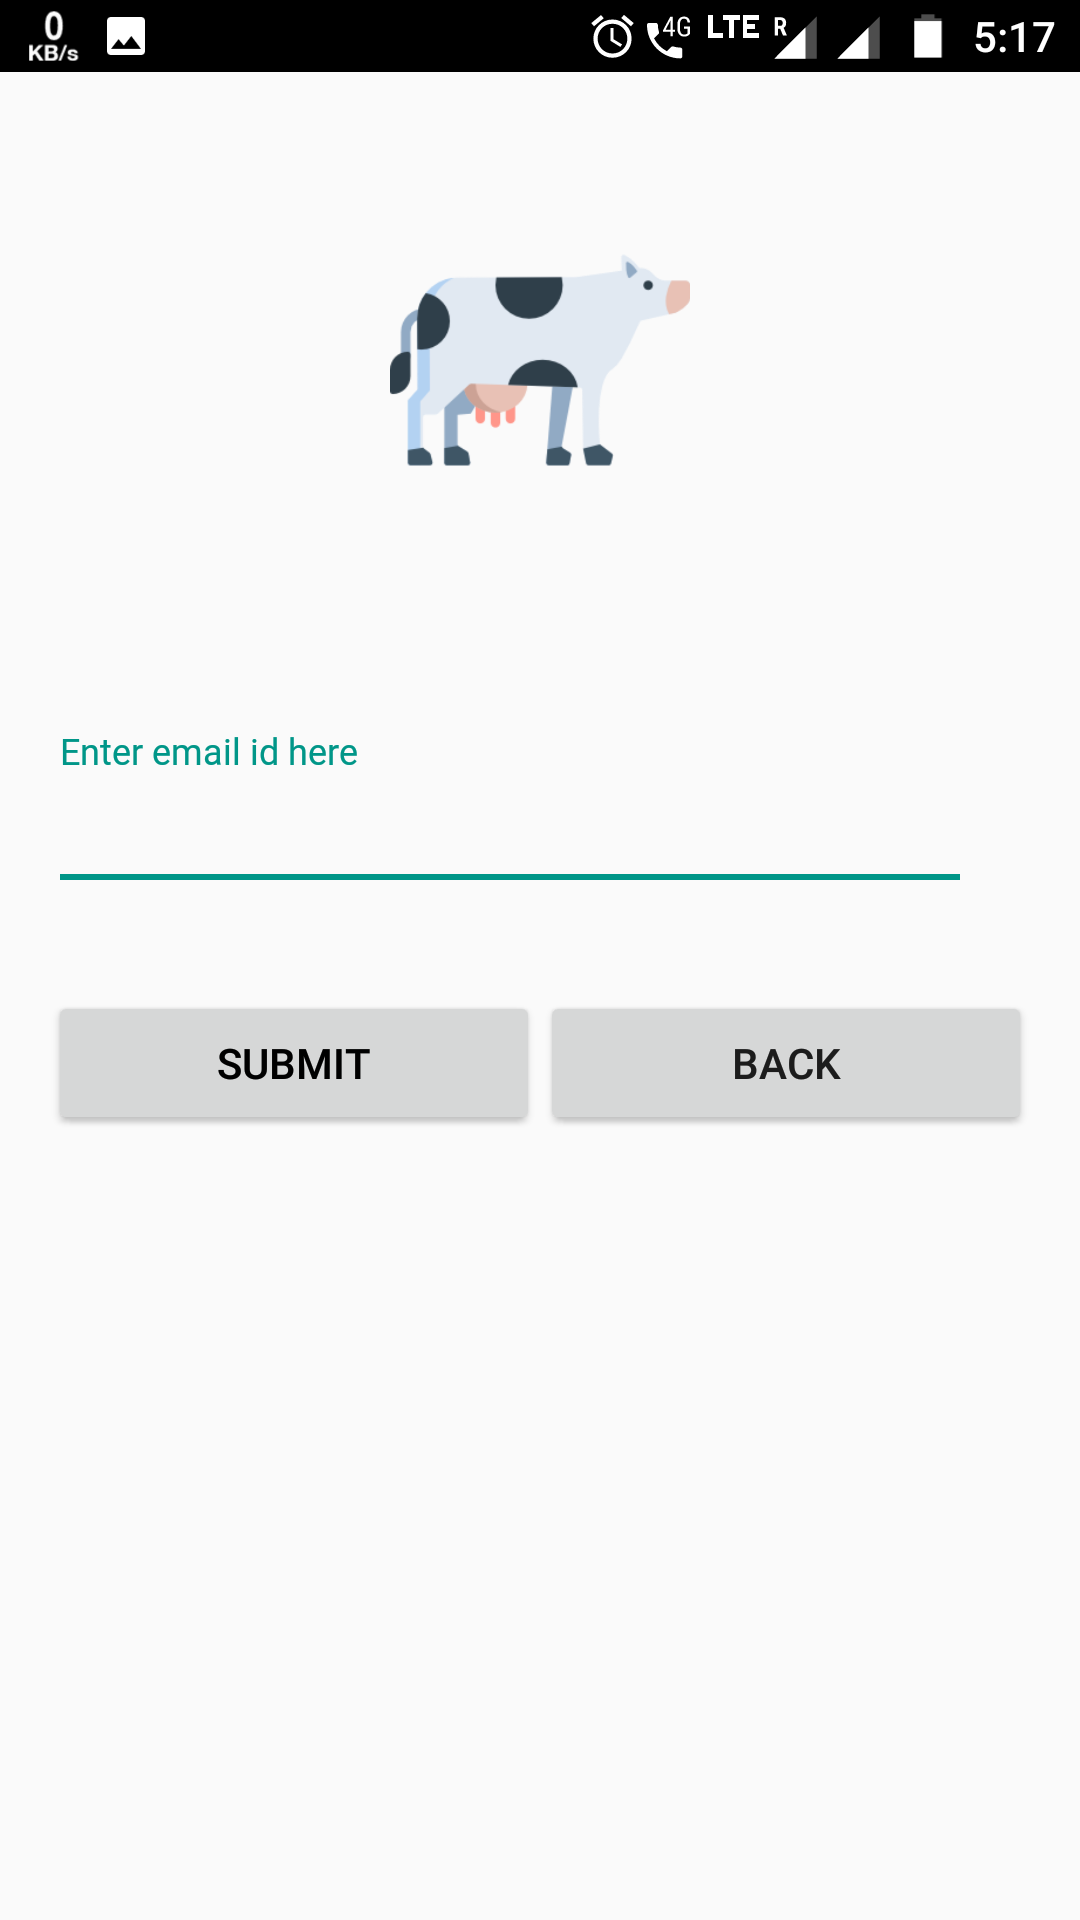
\includegraphics[width=0.7\linewidth]{s03}
	\caption{Forgot Password activity}
\end{figure}
\begin{text}
	\\
	\\
	\\
\end{text}
If you haven't entered email in correct format, you will get an error saying "Enter a valid email address".
\begin{figure}[h]
	\centering
	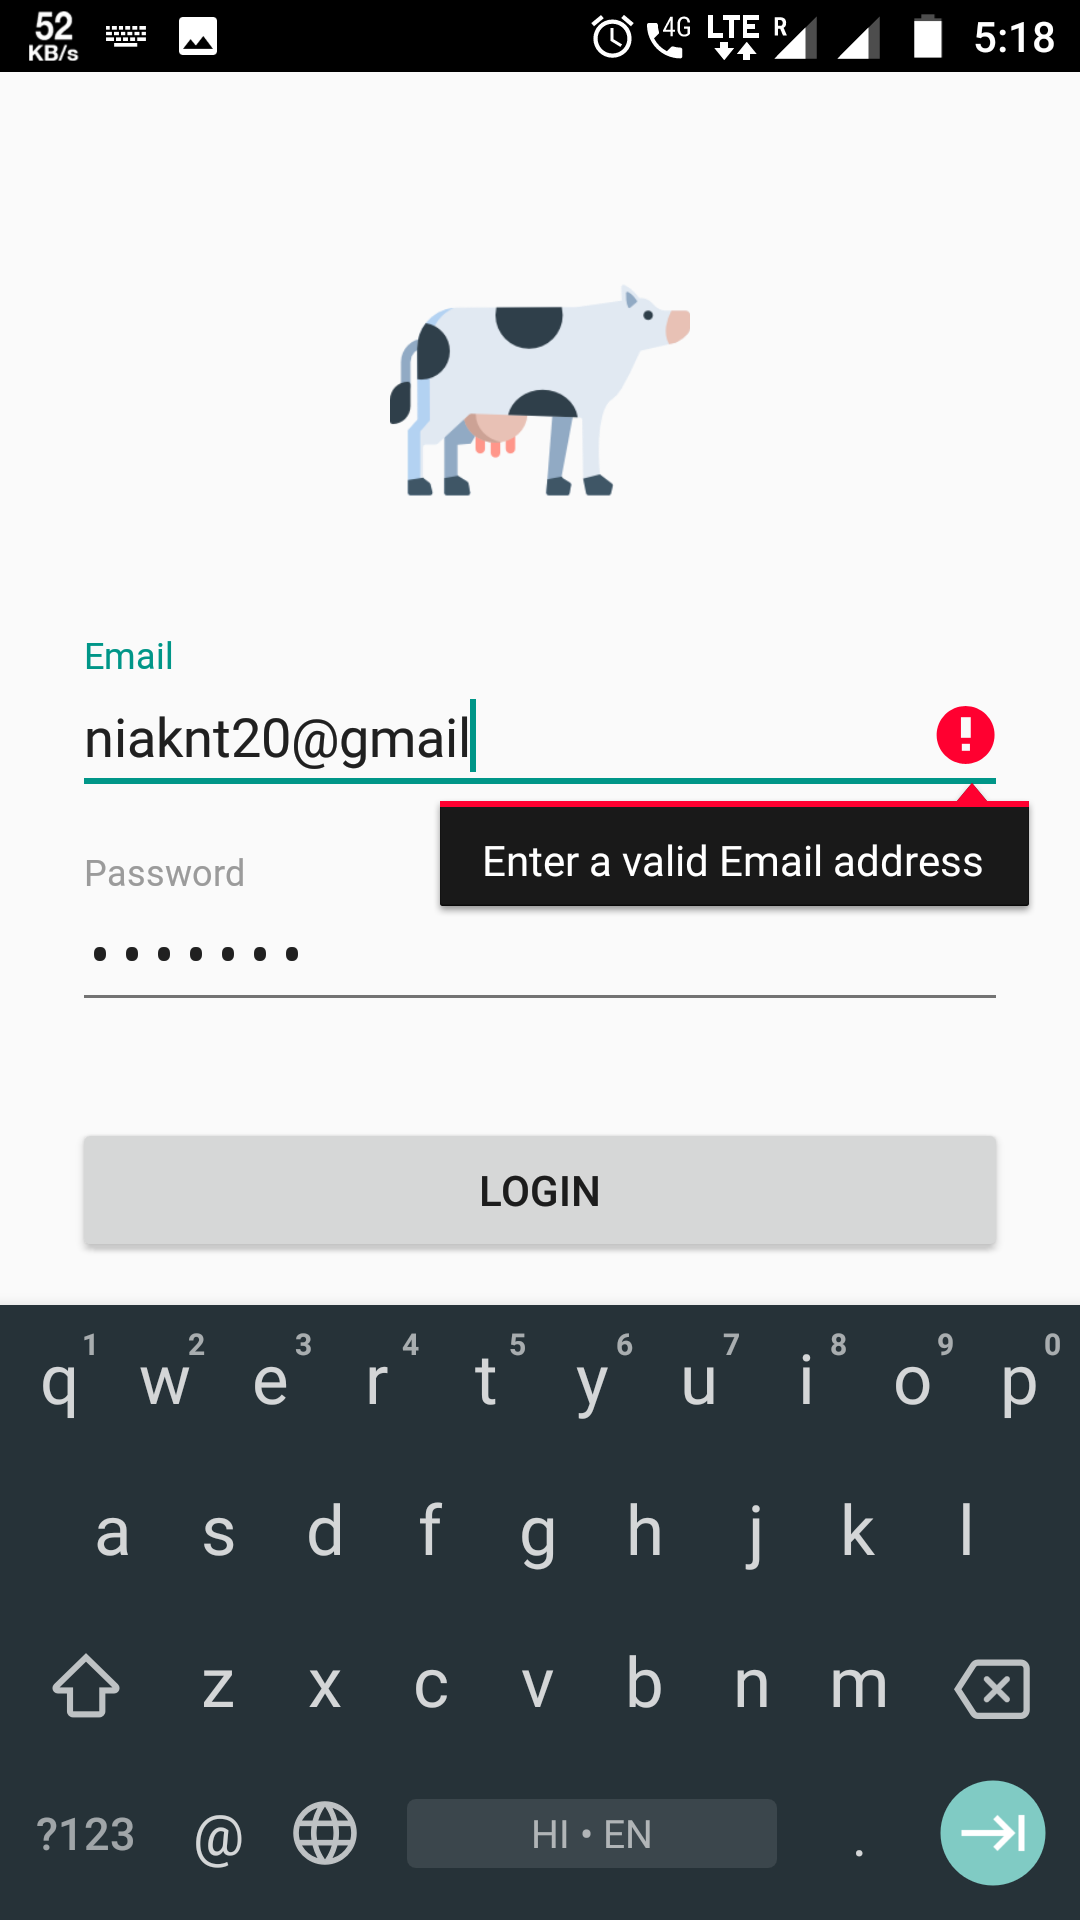
\includegraphics[width=0.7\linewidth]{s04}
	\caption{Validation in Email}
\end{figure}
\begin{text}
	\\
	\\
	\\
	\\
\end{text}
If your password is blank or less than 4 or greater than 10, it will show error.
\begin{figure}[h]
	\centering
	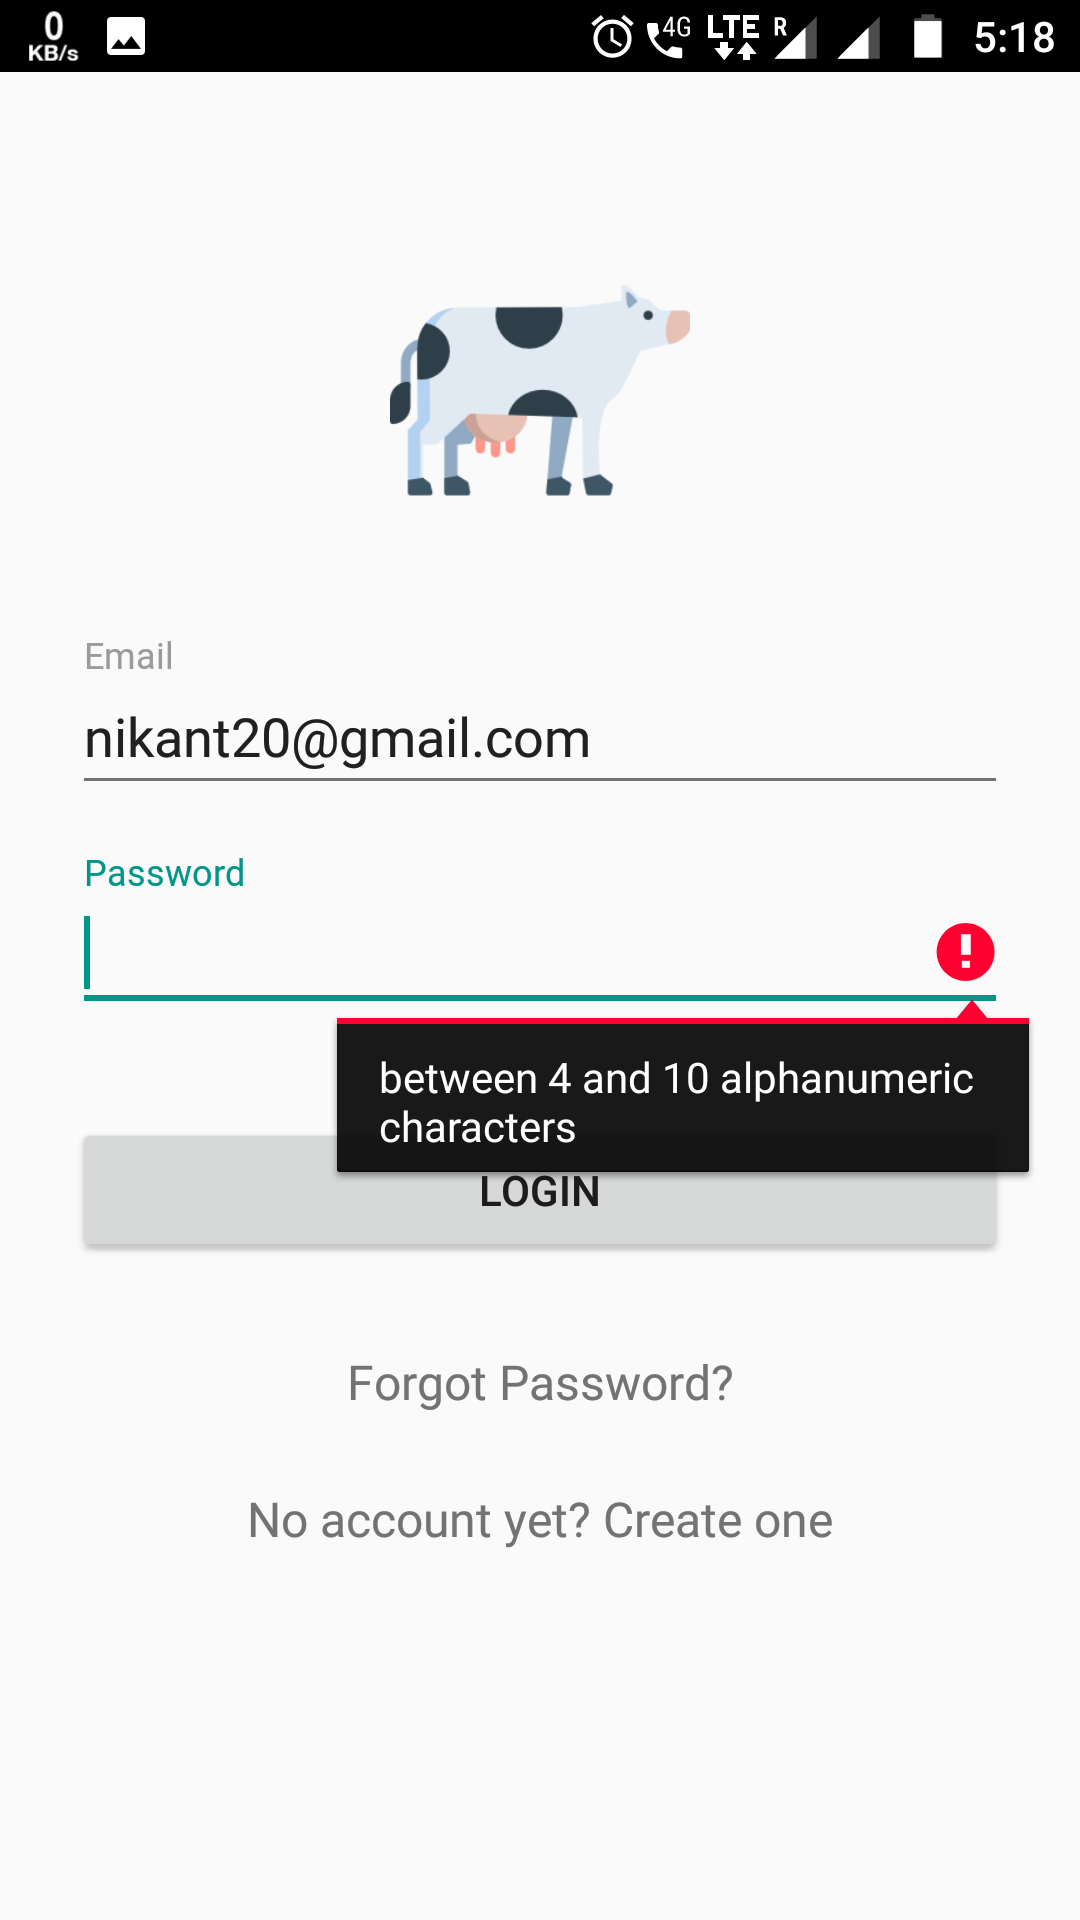
\includegraphics[width=0.7\linewidth]{s05}
	\caption{Validation in Password Field}
\end{figure}
\begin{text}
	\\
	\\
	\\
	\\
\end{text}
If your are a new user, after sign up you will get a blank activity like this.
\begin{figure}[h]
	\centering
	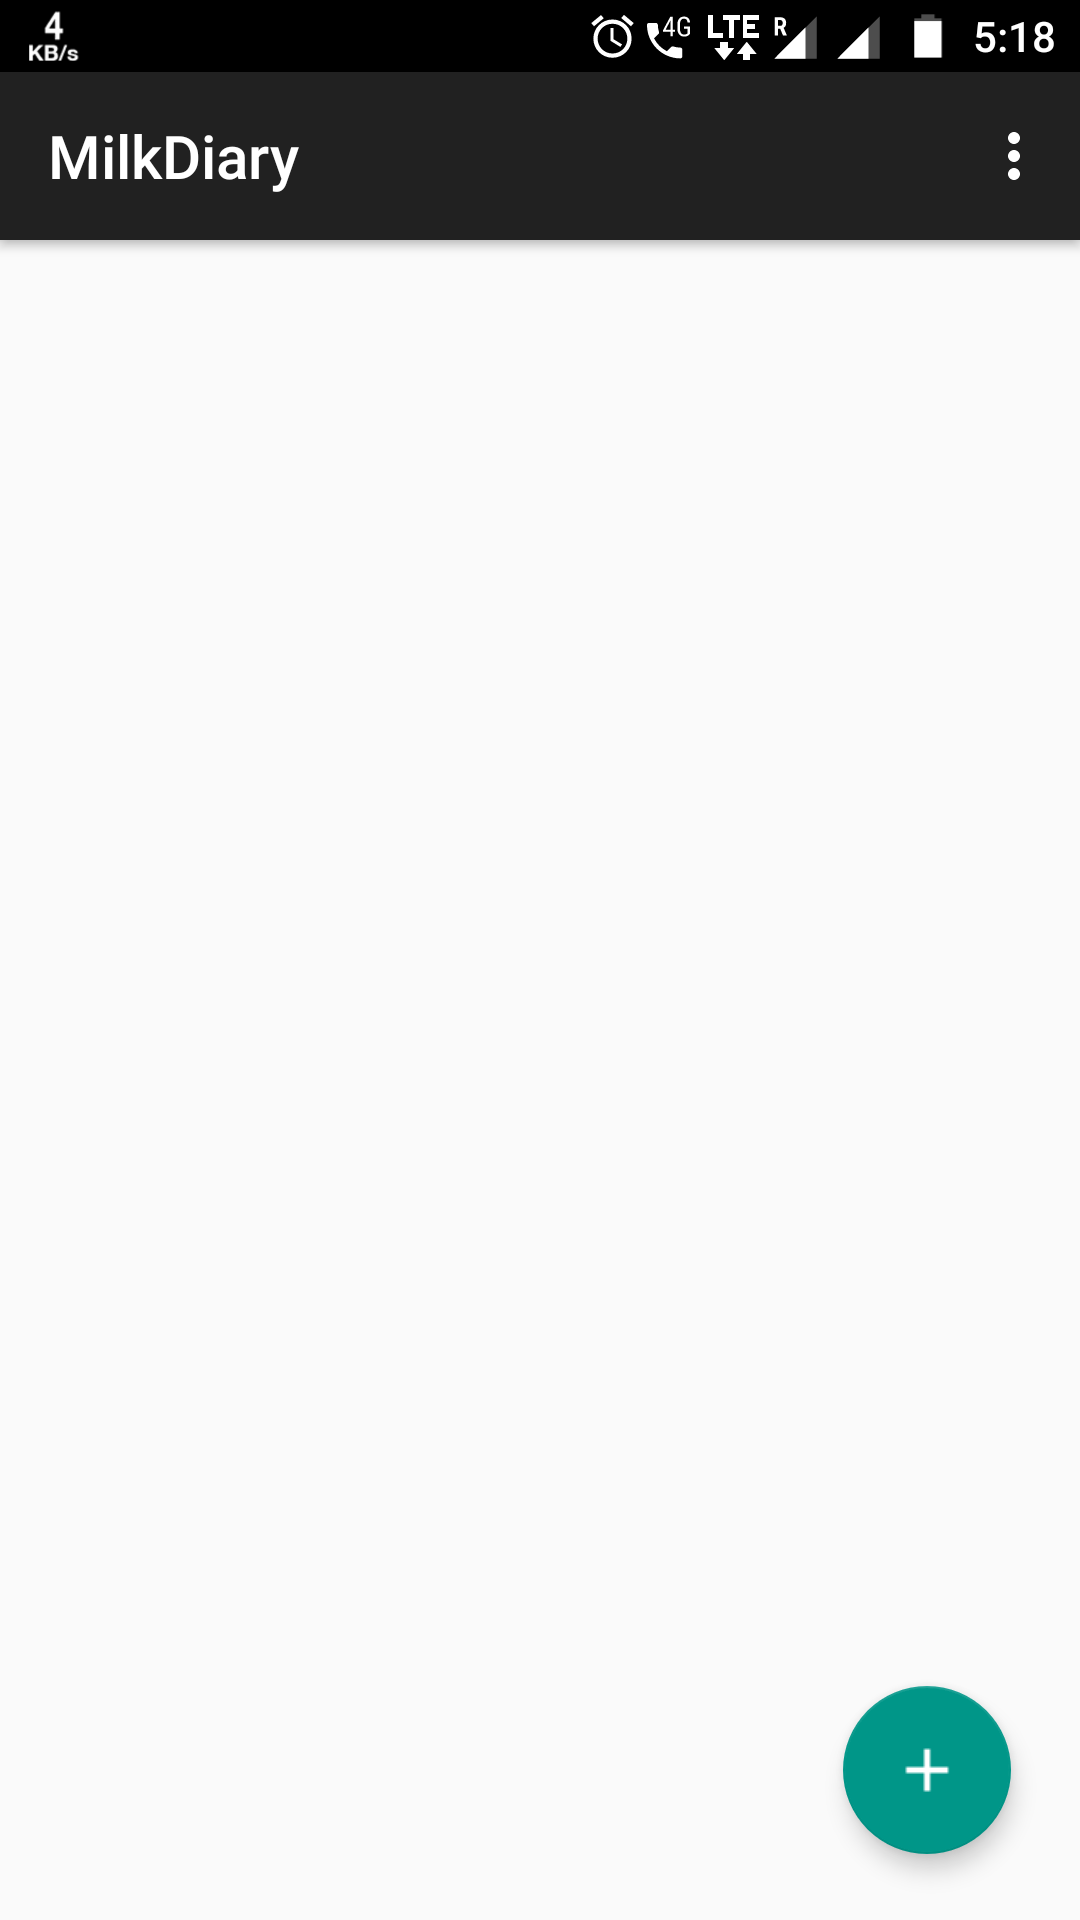
\includegraphics[width=0.7\linewidth]{s06}
	\caption{Blank Activity for new Milkman}
\end{figure}
\begin{text}
	\\
	\\
	\\
	\\
\end{text}
After clicking on a Floating action bar, you will get an activity to add user. Something Like this:
\begin{figure}[h]
	\centering
	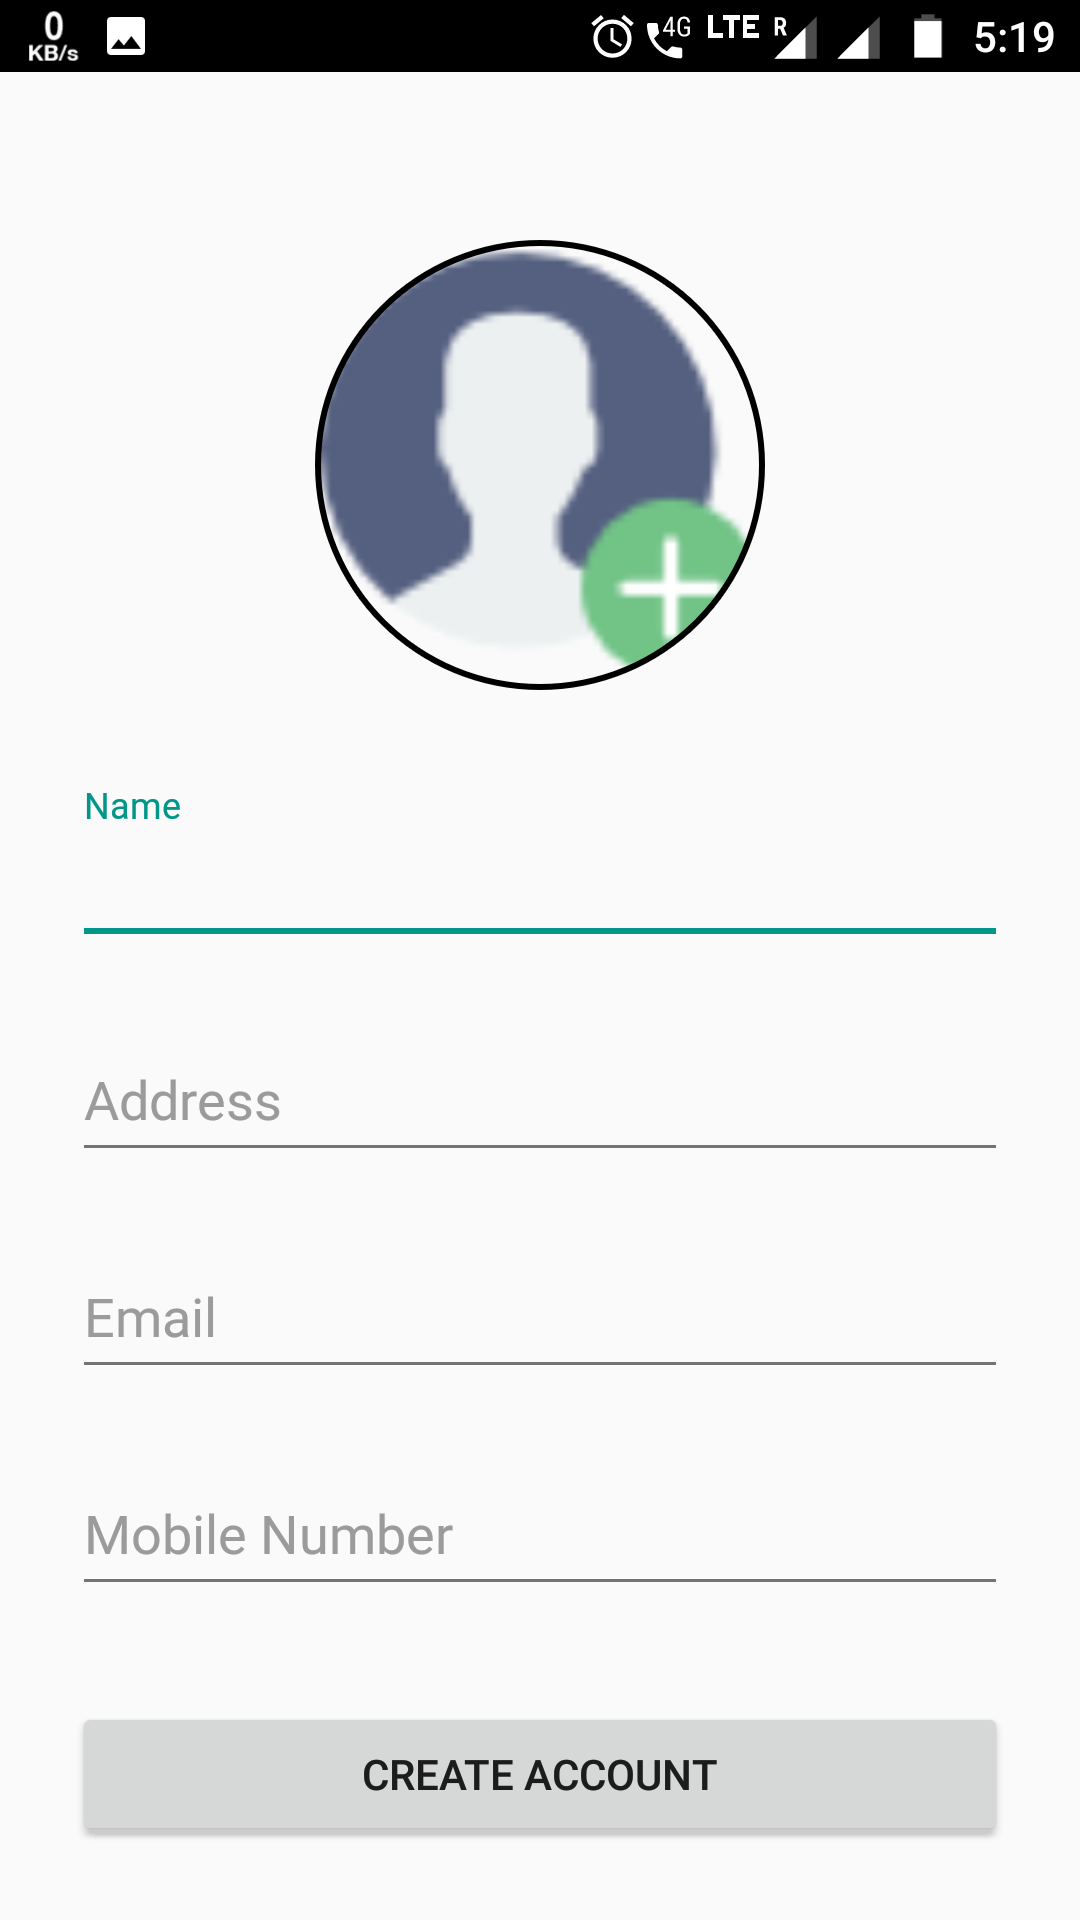
\includegraphics[width=0.7\linewidth]{s07}
	\caption{Add new User Activity}
\end{figure}
\begin{text}
	\\
	\\
	\\
	\\
\end{text}
After adding user, you will get details of user. Something Like this:
\begin{figure}[h]
	\centering
	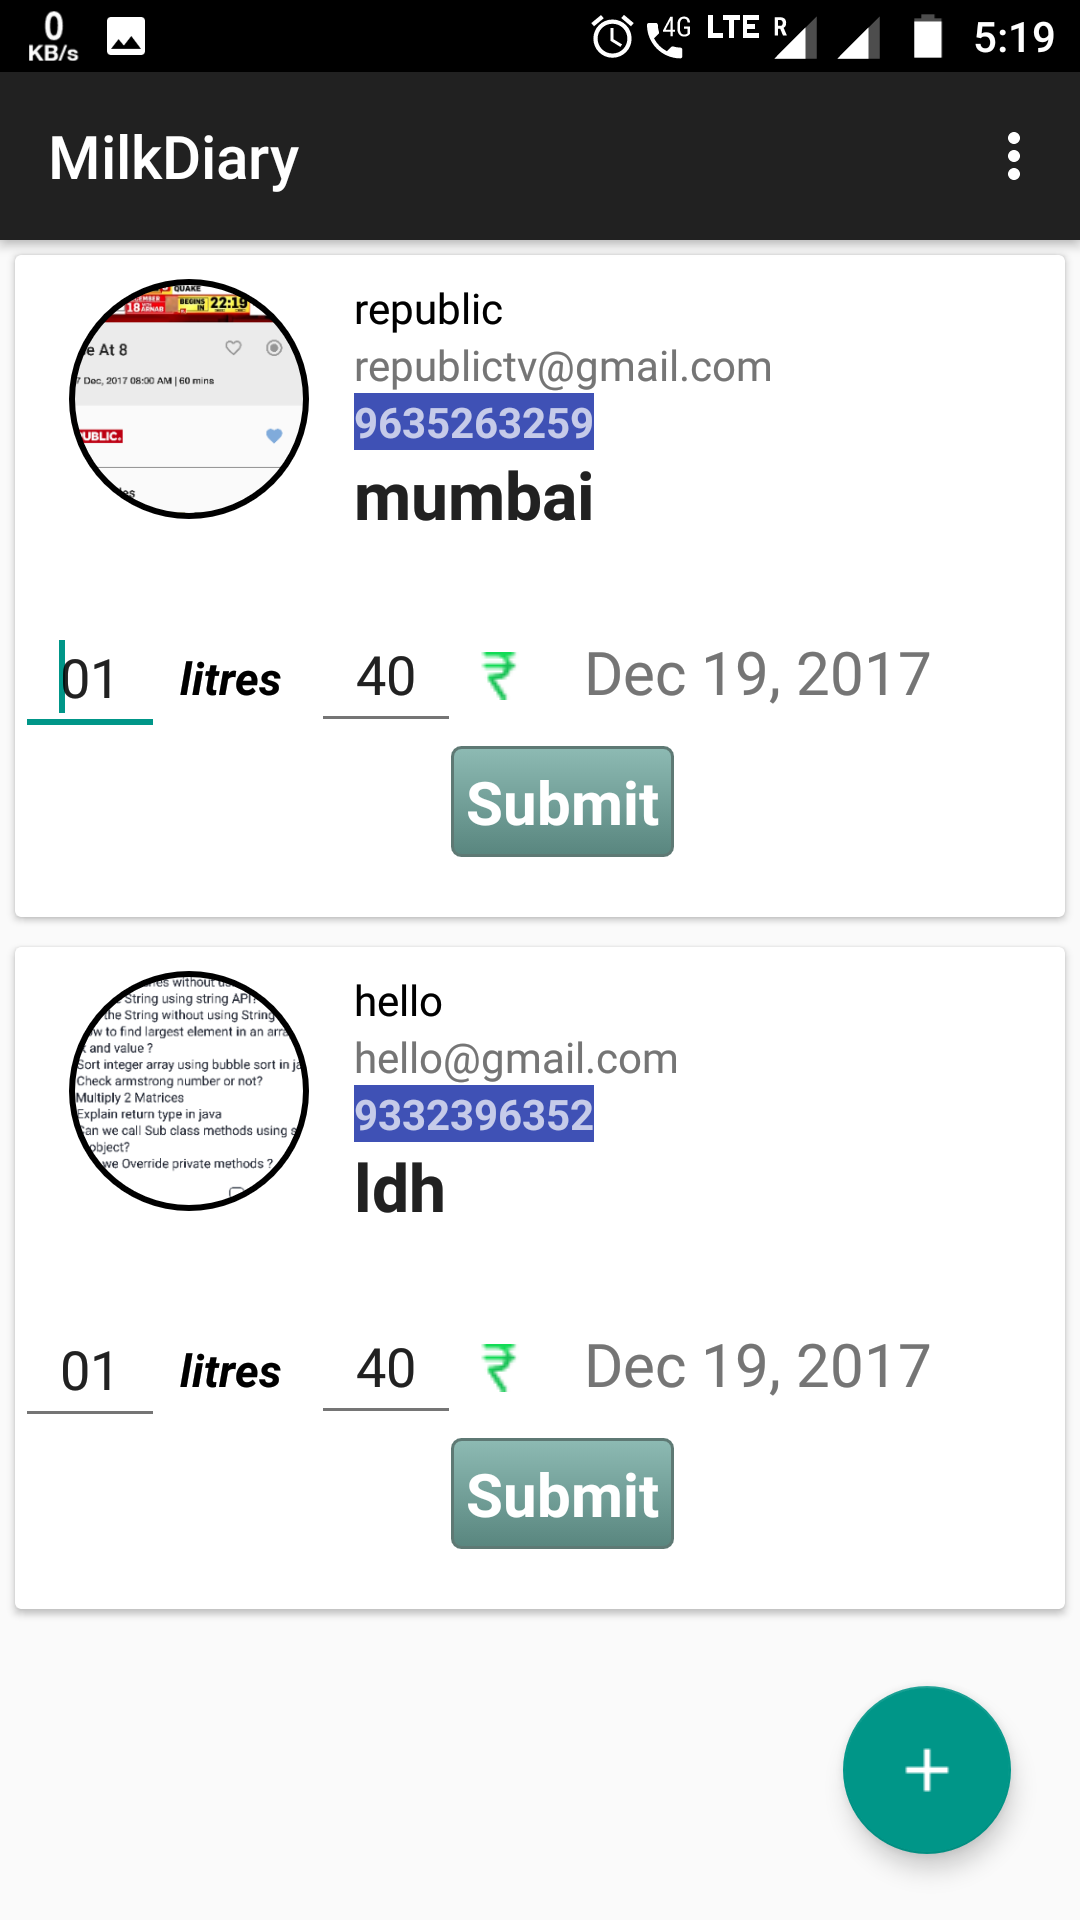
\includegraphics[width=0.7\linewidth]{s08}
	\caption{Add new User Activity}
\end{figure}
\begin{text}
	\\
	\\
	\\
	\\
\end{text}
If u want to logout. there is an option in options menu.
\begin{figure}[h]
	\centering
	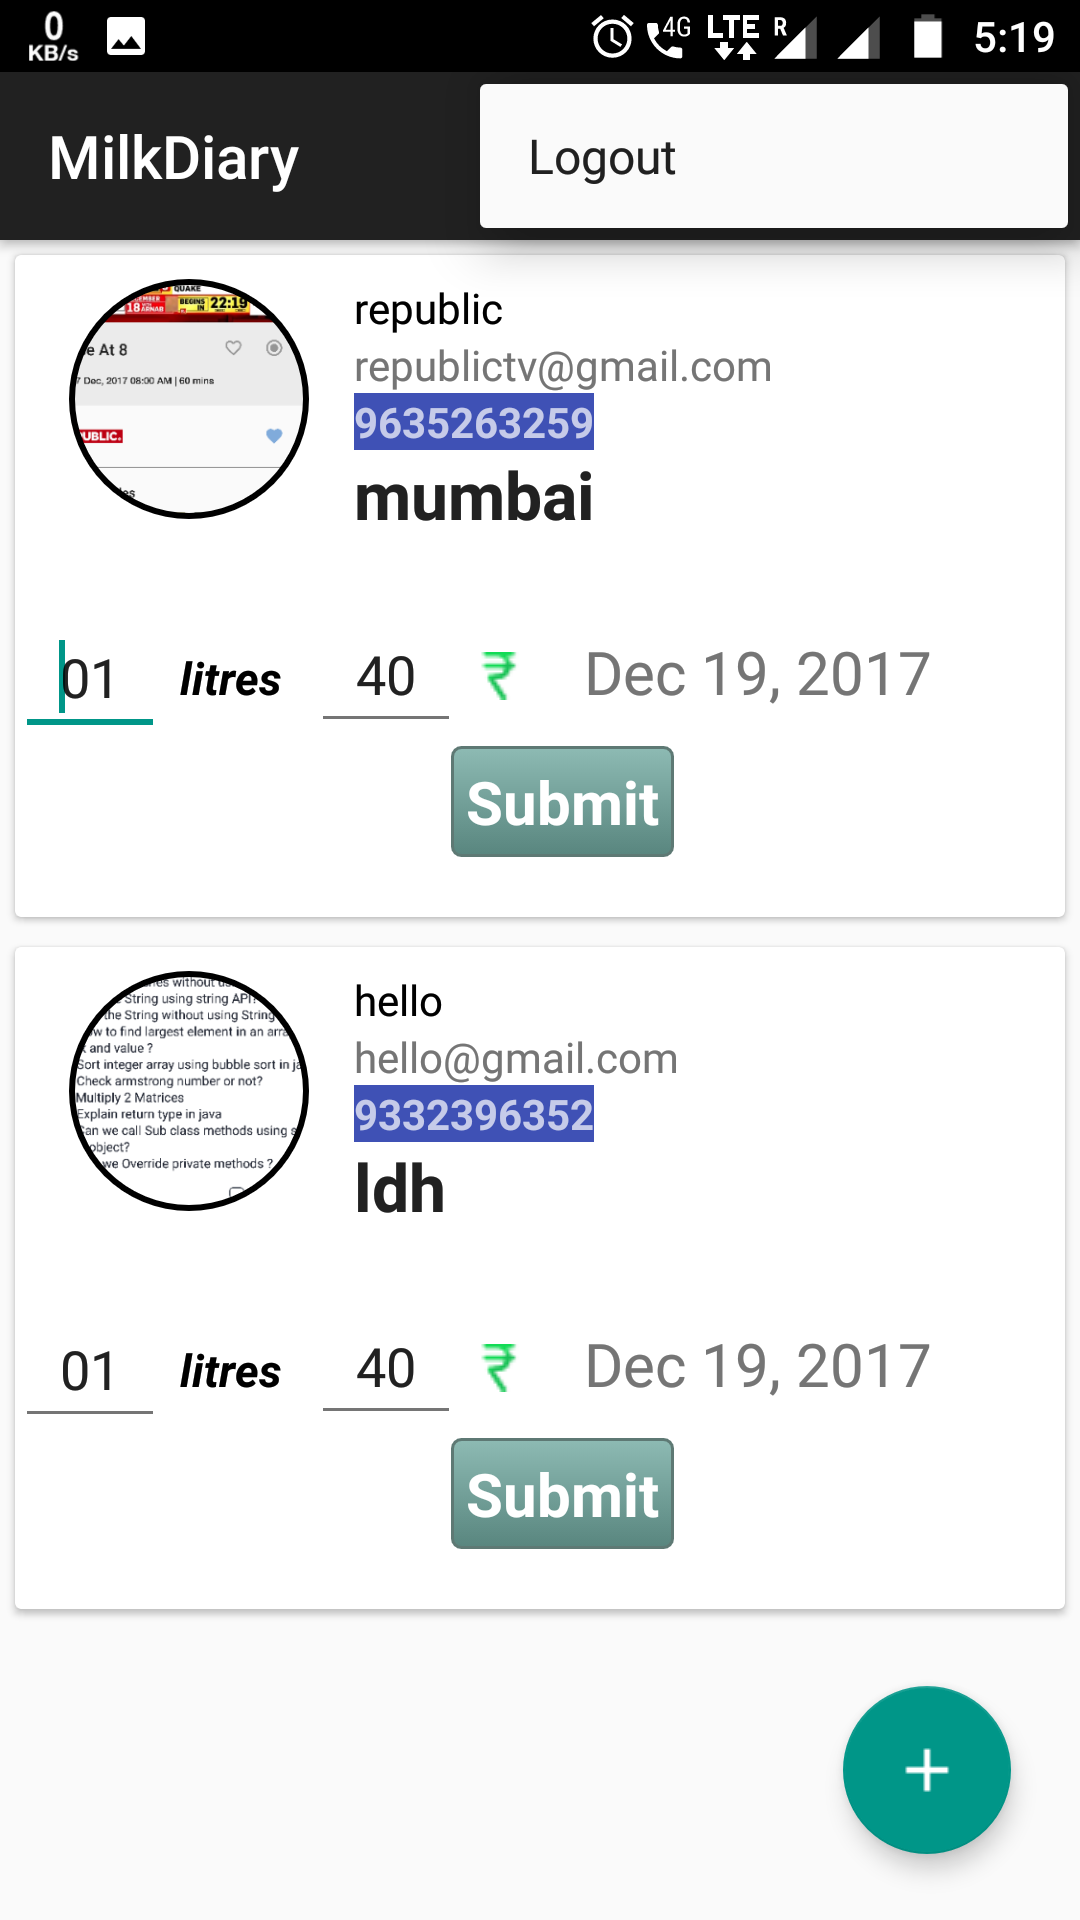
\includegraphics[width=0.7\linewidth]{s09}
	\caption{Logout option Button}
\end{figure}
\begin{text}
	\\
	\\
	\\
	\\
\end{text}
If u want to get Transaction details, click on Name of the customer.
\begin{figure}[h]
	\centering
	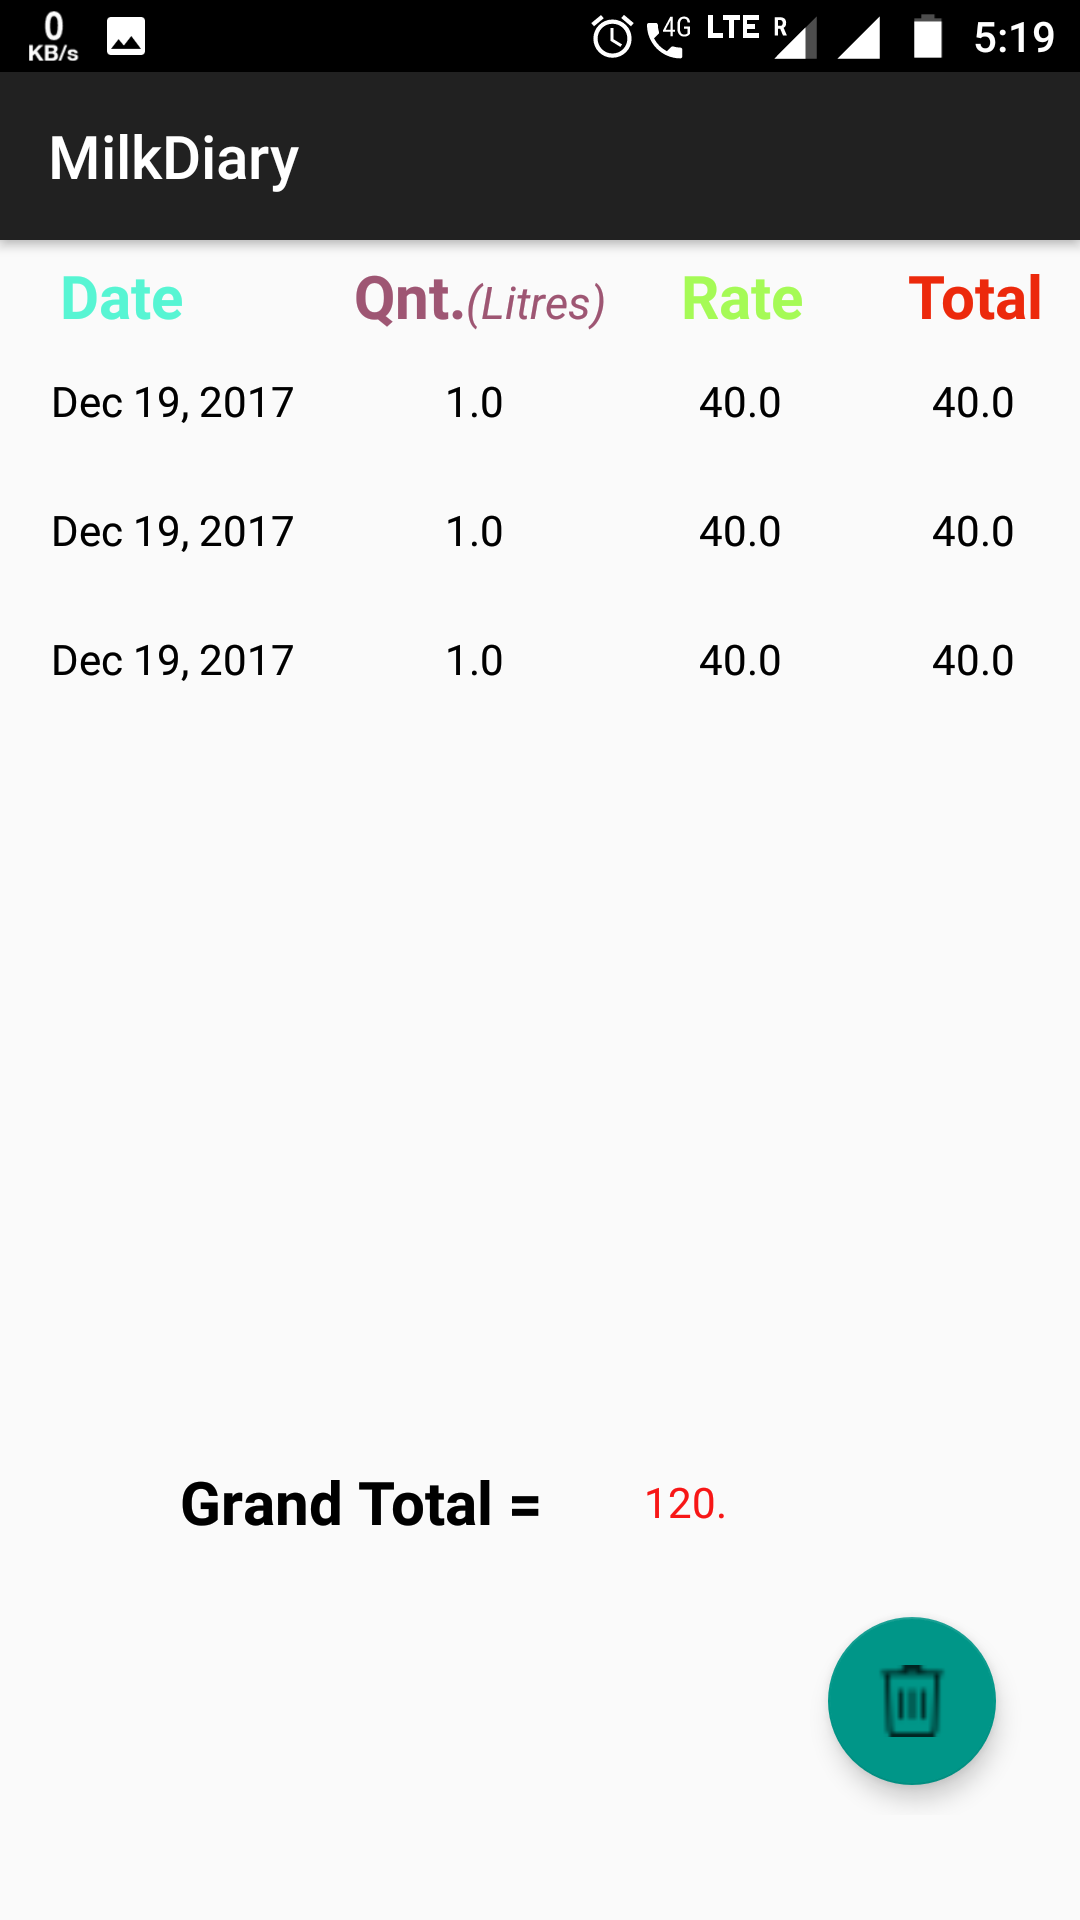
\includegraphics[width=0.7\linewidth]{s10}
	\caption{Transaction History Activity}
\end{figure}
\begin{text}
	\\
	\\
	\\
	\\
\end{text}
If u want to delete Transaction details, click on delete floating action button.
\begin{figure}[h]
	\centering
	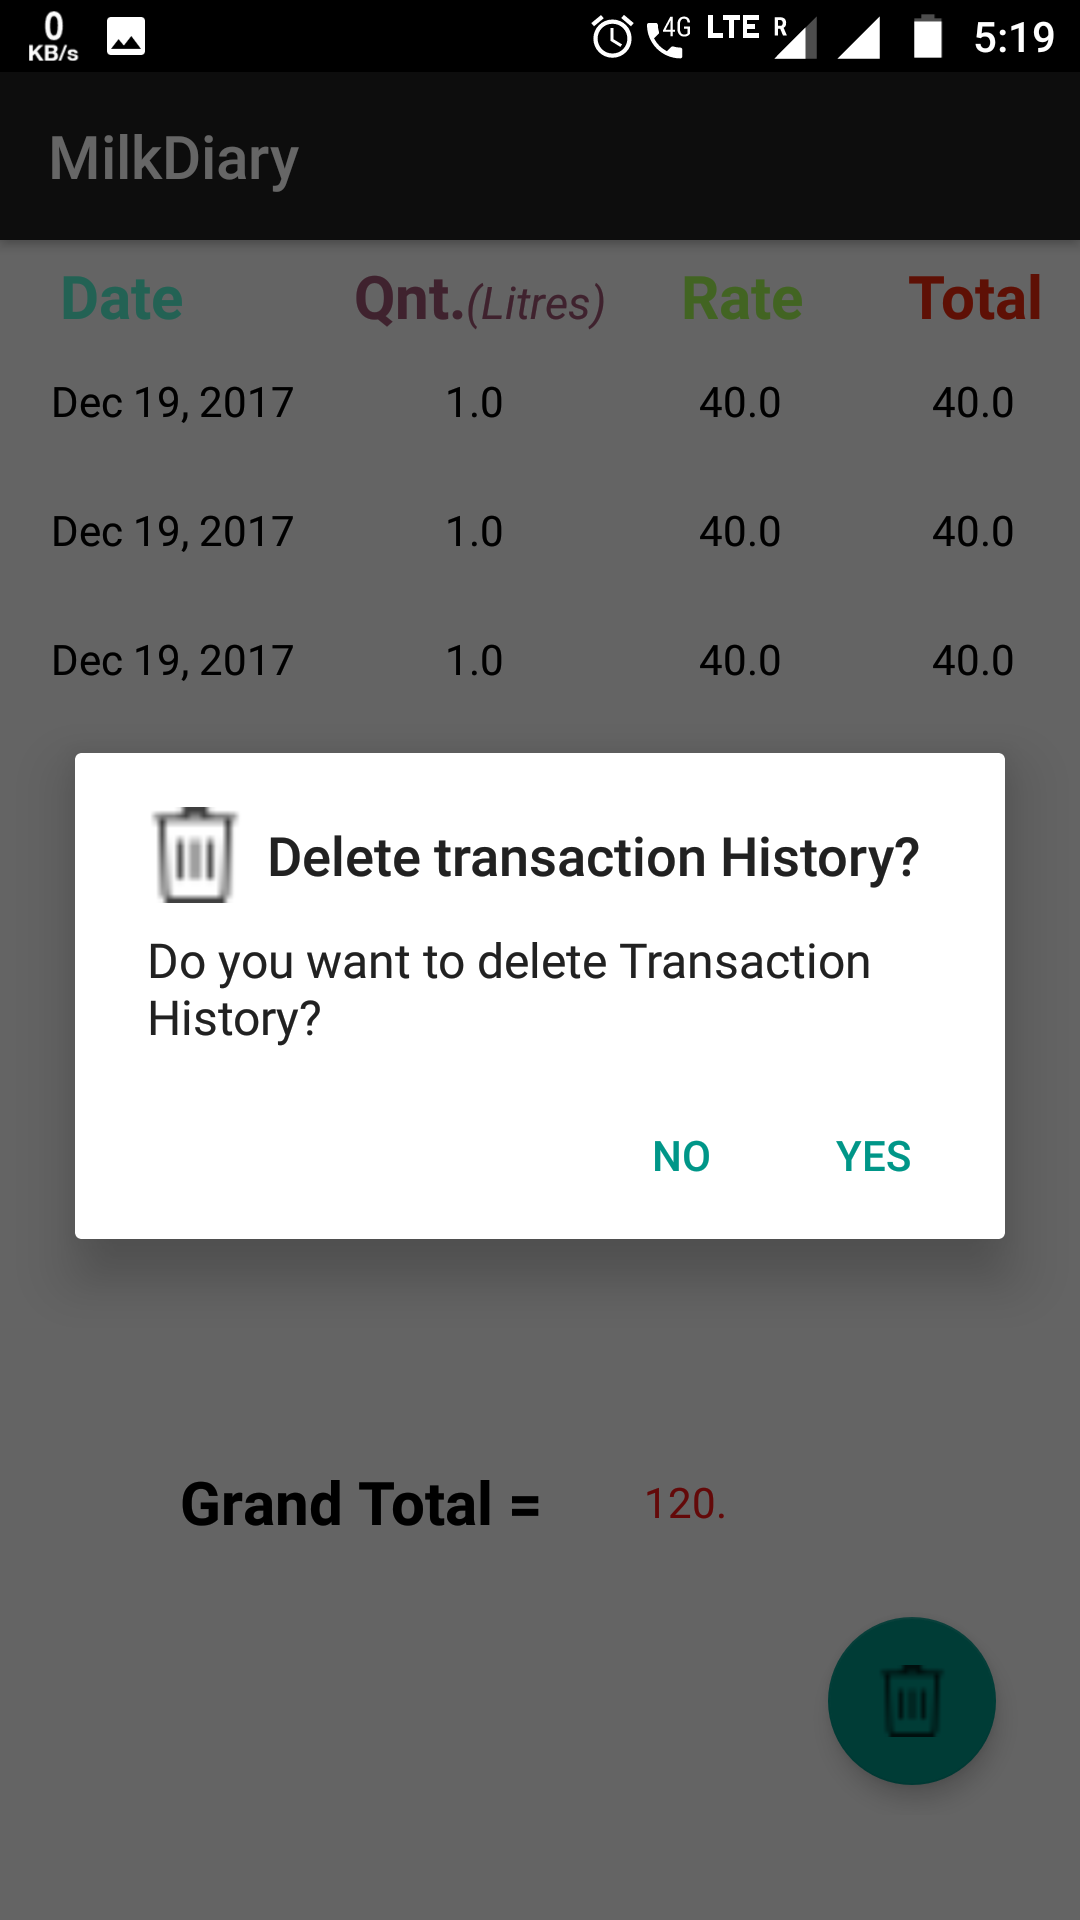
\includegraphics[width=0.7\linewidth]{s11}
	\caption{Transaction History Delete Dialog}
\end{figure}
\begin{text}
	\\
	\\
	\\
	\\
\end{text}

\section{Testing}
Software testing is a critical element of the ultimate review of specification design and coding. Testing of software leads to the uncovering of errors in the software functional and
performance requirements are met. Testing also provides a good indication of software reliability and software quality as a whole. The result of different phases of testing are evaluated and then compared with the expected results. If the errors are uncovered they are debugged and corrected. A strategy approach to software testing has the generic characteristics:
\begin{itemize}
	\item Testing begins at the module level and works outwards towards the integration of
	the entire computer based system.
	\item Testing and debugging are different activities, but debugging must be accommodated in the testing strategy.
	\item Different testing techniques are appropriate at different points of time.
\end{itemize}
Testing of the app is done by JUnit tester provided inbuilt in the android studio.
\\
The app is also tested in realtime environment.\\
It has passed all the tests conducted by Junit and in realtime sucessfully.
\\
The app has also been tested on custom user inputs.
\subsection{Unit Testing in Android}
A unit test verifies in isolation the functionality of a certain component. For example, assume a button in an Android activity is used to start another activity. A unit test would determine, if the corresponding intent was issued, not if the second activity was started.
A unit tests for an Android application can be:
\begin{itemize}
	\item local unit test - which runs on the JVM
	\itemAndroid unit test - which runs on the Android runtime
\end{itemize}
If they run on the JVM, they are executed against a modified version of the android.jar Android library. In this version all final modifiers have been stripped off. This makes it easier to use mocking libraries, like Mockito.
The local unit tests of an Android project should be located in the app/src/test folder.
\subsection{Required dependencies in the Gradle build file}
To use JUnit tests for your Android application, you need to add it as dependency to your Gradle build file.\\
dependencies {
	// Unit testing dependencies\\
	testCompile 'junit:junit:4.12'\\
	// Set this dependency if you want to use the Hamcrest matcher library\\
	testCompile 'org.hamcrest:hamcrest-library:1.3'\\
	// more stuff, e.g., Mockito\\
\subsection{Writing tests to run on the Android device}
The Android testing API provides hooks into the Android component and application life cycle. These hooks are called the instrumentation API and allow your tests to control the life cycle and user interaction events.

Under normal circumstances your application cannot control the life cycle events and the user drives the application. For example, if Android creates your activity the onCreate() method is called. Or if the user presses a button your corresponding code is called. Via instrumentation you can control these events via your test code. For example, your instrumentation test can start the activity. Afterwards, it can call the finish() and restart the activity to test if the instance state of the activity is correctly restored.

Instrumented unit tests are unit tests that run on Android devices and emulators instead of running on the Java virtual machine. These tests have access to the real device and its resources and are useful to unit test functionality which cannot be easily mocked by mocking frameworks. An example is a test which validates a Parcelable implementation.

An instrumentation-based test class allows you to send key events (or touch events) to the application under test.	
}
\chapter{Conclusion and Future Scope}\hrule
\label{Chapter:5}
% =====================================================================================================
\section{Conclusion}
The product which we developed was implemented and tested with data and were found to be error free. Also, it is found that the product will work successfully. We tried to make the product maximum user friendly. All the necessary validations are carried out in this project, so that any kind of users can make use of this product and a necessary message makes them conscious of the error they have made. This product is developed keeping scalability in mind. Additional modules can be easily added when necessary. The software is developed with modular approach. All modules in this system have been tested separately and put together to form the main system. Finally the system is tested with data and everything worked successfully.
\section{Future Scope}
The app has been developed keeping in mind of future feature additions.\\
The app can be integrated with BHIM UPI in near future to get and recieve payments.\\
The App has main moto to increase revenue of MilkMan and make them earn money more in less time. I hope,the App will achieve its aim of development and will generate a great revenue for developer and MilkMan.
\chapter{Refrences}\hrule
\label{Chapter:6}
% =====================================================================================================
\begin{enumerate}
	\item http://www.vogella.com/tutorials/android.html [accesed on 14/10/2017].
	\item https://www.tutorialspoint.com/android/ [accesed on 21/10/2017].
	\item https://developers.google.com/maps/documentation/android-api/marker [accesed on 02/11/2017].
	\item http://www.javatpoint.com/android-tutorial [accesed on 05/11/2017]
	\item http://www.vogella.com/tutorials/AndroidGoogleMaps/article.html [accesed on \\10/11/2017].
	\item http://android-developers.blogspot.in/search?updated-min=\\2016-01-01T00:00:00-08:00updated-max=2017-01-01T00:00:00-08:00max-results=50 [accesed on 12/11/2017].
	\item 
	http://www.vogella.com/tutorials/AndroidTesting/article.html
	[accesed on 15/11/2017].
	\item 
	https://www.sharelatex.com/learn/Lists [accessed on 18/11/2017].
	\item 
	https://stackoverflow.com/questions/41550558/firebase-authentication-depending-on-custom-user-type [accessed on 20/11/2017].
	\item 
	https://stackoverflow.com/questions/27187725/retrieving-specific-data-from-firebase-android [accessed on 22/11/2017].
	\item 
	https://stackoverflow.com/questions/14963776/get-users-by-name-property-using-firebase [accessed on 30/11/2017].
	\item
	https://stackoverflow.com/questions/43374077/i-want-to-retrieve-all-users-uid-from-firebase-user-array-and-store-it-into-arr [accessed on 05/12/2017].
	\item 
	https://stackoverflow.com/questions/38263336/firebase-ui-recyclerview-onclick [accessed on 10/12/2017].
	\item 
	https://www.youtube.com/watch?v=xEHHdpxW7iA&t=374s [accessed on 15/12/2017].
\end{enumerate}